\documentclass[sigconf]{acmart}
\usepackage{booktabs} % For formal tables
\usepackage{listings}
\usepackage[linesnumbered]{algorithm2e}
\usepackage[utf8]{inputenc}
\usepackage{multirow}
\usepackage{color}
\usepackage{pgfplots}
\usepackage{rotating}
\usepackage{pdflscape}
\usepackage{float}
\usepackage{amssymb}
\usepackage{flushend}

\newcommand{\red}[1]{\textcolor{red}{#1}}
\newcommand{\wahab}[1]{\textcolor{blue}{\\ \\Wahab: #1}}
\newcommand{\mathieu}[1]{\textcolor{blue}{\\ \\Mathieu: #1}}

\usepackage[skip=5pt]{caption}

\usepackage{amssymb,amsmath}
\usepackage{ifxetex,ifluatex}
\usepackage{fixltx2e} % provides \textsubscript

\ifnum 0\ifxetex 1\fi\ifluatex 1\fi=0 % if pdftex
  \usepackage[T1]{fontenc}
  \usepackage[utf8]{inputenc}
\else % if luatex or xelatex
  \ifxetex
    \usepackage{mathspec}
    \usepackage{xltxtra,xunicode}
  \else
    \usepackage{fontspec}
  \fi
  \defaultfontfeatures{Mapping=tex-text,Scale=MatchLowercase}
  \newcommand{\euro}{€}


\fi
% use upquote if available, for straight quotes in verbatim environments
\IfFileExists{upquote.sty}{\usepackage{upquote}}{}
% use microtype if available
\IfFileExists{microtype.sty}{%
\usepackage{microtype}
\UseMicrotypeSet[protrusion]{basicmath} % disable protrusion for tt fonts
}{}


\hypersetup{breaklinks=true,
            bookmarks=true,
            pdfauthor={},
            pdftitle={CLEVER: Combining Code Metrics with Clone Detection for Just-In-Time Fault Prevention and Resolution in Large Industrial Projects},
            colorlinks=true,
            citecolor=blue,
            urlcolor=blue,
            linkcolor=magenta,
            pdfborder={0 0 0}}
\urlstyle{same}  % don't use monospace font for urls




\usepackage{color}
\usepackage{fancyvrb}
\newcommand{\VerbBar}{|}
\newcommand{\VERB}{\Verb[commandchars=\\\{\}]}
\DefineVerbatimEnvironment{Highlighting}{Verbatim}{commandchars=\\\{\}}
% Add ',fontsize=\small' for more characters per line
\newenvironment{Shaded}{}{}
\newcommand{\KeywordTok}[1]{\textcolor[rgb]{0.00,0.44,0.13}{\textbf{{#1}}}}
\newcommand{\DataTypeTok}[1]{\textcolor[rgb]{0.56,0.13,0.00}{{#1}}}
\newcommand{\DecValTok}[1]{\textcolor[rgb]{0.25,0.63,0.44}{{#1}}}
\newcommand{\BaseNTok}[1]{\textcolor[rgb]{0.25,0.63,0.44}{{#1}}}
\newcommand{\FloatTok}[1]{\textcolor[rgb]{0.25,0.63,0.44}{{#1}}}
\newcommand{\ConstantTok}[1]{\textcolor[rgb]{0.53,0.00,0.00}{{#1}}}
\newcommand{\CharTok}[1]{\textcolor[rgb]{0.25,0.44,0.63}{{#1}}}
\newcommand{\SpecialCharTok}[1]{\textcolor[rgb]{0.25,0.44,0.63}{{#1}}}
\newcommand{\StringTok}[1]{\textcolor[rgb]{0.25,0.44,0.63}{{#1}}}
\newcommand{\VerbatimStringTok}[1]{\textcolor[rgb]{0.25,0.44,0.63}{{#1}}}
\newcommand{\SpecialStringTok}[1]{\textcolor[rgb]{0.73,0.40,0.53}{{#1}}}
\newcommand{\ImportTok}[1]{{#1}}
\newcommand{\CommentTok}[1]{\textcolor[rgb]{0.38,0.63,0.69}{\textit{{#1}}}}
\newcommand{\DocumentationTok}[1]{\textcolor[rgb]{0.73,0.13,0.13}{\textit{{#1}}}}
\newcommand{\AnnotationTok}[1]{\textcolor[rgb]{0.38,0.63,0.69}{\textbf{\textit{{#1}}}}}
\newcommand{\CommentVarTok}[1]{\textcolor[rgb]{0.38,0.63,0.69}{\textbf{\textit{{#1}}}}}
\newcommand{\OtherTok}[1]{\textcolor[rgb]{0.00,0.44,0.13}{{#1}}}
\newcommand{\FunctionTok}[1]{\textcolor[rgb]{0.02,0.16,0.49}{{#1}}}
\newcommand{\VariableTok}[1]{\textcolor[rgb]{0.10,0.09,0.49}{{#1}}}
\newcommand{\ControlFlowTok}[1]{\textcolor[rgb]{0.00,0.44,0.13}{\textbf{{#1}}}}
\newcommand{\OperatorTok}[1]{\textcolor[rgb]{0.40,0.40,0.40}{{#1}}}
\newcommand{\BuiltInTok}[1]{{#1}}
\newcommand{\ExtensionTok}[1]{{#1}}
\newcommand{\PreprocessorTok}[1]{\textcolor[rgb]{0.74,0.48,0.00}{{#1}}}
\newcommand{\AttributeTok}[1]{\textcolor[rgb]{0.49,0.56,0.16}{{#1}}}
\newcommand{\RegionMarkerTok}[1]{{#1}}
\newcommand{\InformationTok}[1]{\textcolor[rgb]{0.38,0.63,0.69}{\textbf{\textit{{#1}}}}}
\newcommand{\WarningTok}[1]{\textcolor[rgb]{0.38,0.63,0.69}{\textbf{\textit{{#1}}}}}
\newcommand{\AlertTok}[1]{\textcolor[rgb]{1.00,0.00,0.00}{\textbf{{#1}}}}
\newcommand{\ErrorTok}[1]{\textcolor[rgb]{1.00,0.00,0.00}{\textbf{{#1}}}}
\newcommand{\NormalTok}[1]{{#1}}






\setlength{\emergencystretch}{3em}  % prevent overfull lines
\providecommand{\tightlist}{%
  \setlength{\itemsep}{0pt}\setlength{\parskip}{0pt}}
\setcounter{secnumdepth}{5}


\usepackage{booktabs}
\setcopyright{rightsretained}
\acmConference[MSR'18]{ACM MSR Conference}{May 2018}{Gothemburg, Sweden} 
\acmYear{018}
\copyrightyear{2018}

\acmArticle{4}
\acmPrice{15.00}

\begin{document}

\title{CLEVER: Combining Code Metrics with Clone Detection for Just-In-Time
Fault Prevention and Resolution in Large Industrial Projects\vspace{0.5cm}}

\author{Mathieu Nayrolles}
\affiliation{%
  \institution{La Forge Research Lab, Ubisoft}
  \streetaddress{Montréal, QC, Canada}
}
\email{mathieu.nayrolles@ubisoft.com}
\author{Abdelwahab Hamou-Lhadj}
\affiliation{%
  \institution{ECE Department, Concordia University}
  \streetaddress{Montréal, QC, Canada}
}
\email{wahab.hamou-lhadj@concordia.ca}

\renewcommand{\shorttitle}{Combining Code Metrics With Clone Detection For Faults Prevention and Resolution}

\begin{abstract}
Automatic prevention and resolution of faults is an important research
topic in the field of software maintenance and evolution. Existing
approaches leverage code and process metrics to build metric-based
models that can effectively prevent defect insertion in a software
project. Metrics, however, may vary from one project to another,
hindering the reuse of these models. Moreover, they tend to generate
high false positive rates by classifying healthy commits as risky.
Finally, they do not provide sufficient insights to developers on how to
fix the detected risky commits. In this paper, we propose an approach,
called CLEVER (Combining Levels of Bug Prevention and Resolution
techniques), which relies on a two-phase process for intercepting risky
commits before they reach the central repository. CLEVER was developed
in collaboration with Ubisoft developers. When applied to 12 Ubisoft
systems, the results show that CLEVER can detect risky commits with 79\%
precision and 65\% recall, which outperforms the performance of
Commit-guru, a recent approach that was proposed in the literature. In
addition, CLEVER is able to recommend qualitative fixes to developers on
how to fix risky commits in 66.7\% of the cases.
\end{abstract}

%
% The code below should be generated by the tool at
% http://dl.acm.org/ccs.cfm
% Please copy and paste the code instead of the example below. 
%
\begin{CCSXML}
<ccs2012>
<concept>
<concept_id>10011007.10011074.10011099.10011102.10011103</concept_id>
<concept_desc>Software and its engineering~Software testing and debugging</concept_desc>
<concept_significance>500</concept_significance>
</concept>
<concept>
<concept_id>10011007.10011074.10011111.10011696</concept_id>
<concept_desc>Software and its engineering~Maintaining software</concept_desc>
<concept_significance>300</concept_significance>
</concept>
<concept>
<concept_id>10002951.10003227.10003241.10003243</concept_id>
<concept_desc>Information systems~Expert systems</concept_desc>
<concept_significance>100</concept_significance>
</concept>
</ccs2012>
\end{CCSXML}

\ccsdesc[500]{Software and its engineering~Software testing and debugging}
\ccsdesc[300]{Software and its engineering~Maintaining software}
\ccsdesc[100]{Information systems~Expert systems}

\keywords{Defect Predictions, Fault Fixing, Software Maintenance, Software Evolution}

\maketitle

\section{Introduction}\label{sec:introduction}

Automatic prevention and resolution of faults is an important research
topic in the field of software maintenance and evolution. Effective
approaches can help reduce significantly the cost of maintenance of
software systems, while improving their quality. A particular line of
research focuses on the problem of preventing the introduction of faults
by detecting risky commits (commits that may potentially introduce
faults in the system) before they reach the central code repository. We
refer to this as just-in-time fault detection/prevention [18].

There exist techniques that aim to detect risky commits (e.g., [2, 5,
42]), among which the most recent approach is the one proposed by
Rosen et al. [38]. The authors developed an approach and a
supporting tool, Commit-guru, that relies on building models from
historical commits using code and process metrics (e.g., code
complexity, the experience of the developers, etc.) as main features.
These models are used to classify new commits as risky or not.
Commit-guru has been shown to outperform previous techniques (e.g.,
[19, 25]).

However, Commit-guru and similar tools suffer from a number of
limitations. First, they tend to generate high false positive rates by
classifying healthy commits as risky. The second limitation is that they
do not provide recommendations to developers on how to fix the detected
risky commits. They simply return measurements that are often difficult
to interpret by developers. In addition, they have been mainly validated
using open source systems. Their effectiveness when applied to
industrial systems has yet to be shown.

In this paper, we propose an approach, called CLEVER (Combining Levels
of Bug Prevention and Resolution techniques), that relies on a two-phase
process for intercepting risky commits before they reach the central
repository. The first phase consists of building a metric-based model to
assess the likelihood that an incoming commit is risky or not. This is
similar to existing approaches. The next phase relies on clone detection
to compare code blocks extracted from suspicious risky commits, detected
in the first phase, with those of known historical fault-introducing
commits. This additional phase provides CLEVER with two apparent
advantages over Commit-guru. First, as we will show in the evaluation
section, CLEVER is able to reduce the number of false positives by
relying on code matching instead of mere metrics. The second advantage
is that, with CLEVER, it is possible to use commits that were used to
fix faults introduced by previous commits to suggest recommendations to
developers on how to improve the risky commits at hand. This way, CLEVER
goes one step further than Commit-guru (and similar techniques) by
providing developers with a potential fix for their risky commits.

Another important aspect of CLEVER is its ability to detect risky
commits not only by comparing them to commits of a single project but
also to those belonging to other projects that share common
dependencies. This is important in the context of an industrial setting
where software systems tend to have many dependencies that make them
vulnerable to the same faults.

CLEVER was developed in collaboration with software developers from
Ubisoft La Forge. Ubisoft is one of the world's largest video game
development companies specializing in the design and implementation of
high-budget video games. Ubisoft software systems are highly coupled
containing millions of files and commits, developed and maintained by
more than 8,000 developers scattered across 29 locations in six
continents.

We tested CLEVER on 12 major Ubisoft systems. The results show that
CLEVER can detect risky commits with 79\% precision and 65\% recall,
which outperforms the performance of Commit-guru (66\% precision and
63\% recall) when applied to the same dataset. In addition, 66.7\% of
the proposed fixes were accepted by at least one Ubisoft software
developer, making CLEVER an effective and practical approach for the
detection and resolution of risky commits.

The remaining parts of this paper are organised as follows. In Section
\ref{sec:relwork}, we present related work. Sections \ref{sec:CLEVERT},
\ref{sec:exp} and \ref{sec:result} are dedicated to describing the
CLEVER approach, the case study setup, and the case study results. Then,
Sections \ref{sec:threats} and \ref{sec:conclusion} present the threats
to validity and a conclusion accompanied with future work.

\section{Related Work}\label{sec:relwork}

Our approach, CLEVER, is related to two research areas: defect
prediction and patch generation.

\subsection{File, Module, and Risky Change
Prediction}\label{file-module-and-risky-change-prediction}

Existing studies for predicting risky changes within a repository rely
mainly on code and process metrics. As discussed in the introduction
section, Rosen et al. [38] developed Commit-guru a tool that relies
on building models from historical commits using code and process
metrics (e.g., code complexity, the experience of the developers, etc.)
as the main features. There exist other studies that leverage several
code metric suites such as the CK metrics suite [5] or the Briand's
coupling metrics [2]. These metrics have been used, with success, to
predict defects as shown by Subramanyam \emph{et al.} [42] and
Gyimothy \emph{et al.} [11].

Further improvements to these metrics have been proposed by Nagappan
\emph{et al.} [31, 33] and Zimmerman \emph{et al.} [48, 49] who
used call graphs as the main artifact for computing code metrics with a
static analyzer.

Nagappan \emph{et al.} proposed a technique that uses data mined from
source code repository such as churns to assess the quality of a change
[32]. Hassan \emph{et al} and Ostrand \emph{et al} used past changes
and defects to predict buggy locations [12], [35]. Their methods
rely on various heuristics to identify the locations that are most
likely to introduce a defect. Kim \emph{et al} [24] proposed the bug
cache approach, which is an improved technique over Hassan and Holt's
approach [12]. Rahman and Devanbu found that, in general,
process-based metrics perform as good as code-based metrics [37].

Other studies that aim to predict risky changes use the entropy of a
given change [13, 43] and the size of the change combined with files
being changed [20].

These techniques operate at different levels of the systems and may
require the presence of the entire source code. In addition, the
reliance of metrics may result in high false positives rates. We need a
way to validate whether a suspicious change is indeed risky. In this
paper, we address this issue using a two-phase process that combines the
use of metrics to detect suspicious risky changes, and code matching to
increase the detect accuracy. As we will show in the evaluation section,
CLEVER reduces the number of false positives while keeping good recall.
In addition, CLEVER operates at commit-time for preventing the
introduction of faults before they reach the code repository. Through
interactions with Ubisoft developers, we found that this integrates well
with the workflow of developers.

\subsection{Automatic Patch
Generation}\label{automatic-patch-generation}

One feature of CLEVER is the ability to propose fixes that can help
developers correct the detected risky commit. This is similar in
principle to the work on automatic patch generation. Pan \emph{et al.}
and Kim \emph{et al.} proposed two approaches that extract and apply fix
patterns [22, 36]. Pan \emph{et al.} identified 27 patterns and were
able to fix 45.7\% - 63.6\% of bugs using one of the proposed patterns.
The patterns found by Kim \emph{et al.} are mined from human-written
patches and were able to successfully generate patches for 27 out of 119
bugs. The tool by Kim \emph{et al.}, named PAR, is similar to the second
part of CLEVER where we propose fixes. Our approach also mines potential
fixes from human-written patches found in the historical data. In our
work, we do not generate patches, but instead propose known patches to
developers for further assessment. It has also been shown that patch
generation is useful in understanding and debugging the causes of faults
[44].

Despite the advances in the field of automatic patch generation, this
task remains overly complex. Developers expect from tools high quality
patches that can be safely deployed. Many studies proposed a
classification of what is considered an acceptable quality patch for an
automatically generated patch to be adopted in industry [7, 26, 27].

\section{The CLEVER Approach}\label{sec:CLEVERT}


Figures \ref{fig:CLEVERT1}, \ref{fig:CLEVERT3} and \ref{fig:CLEVERT2}
show an overview of the CLEVER approach, which consists of two parallel
processes.

In the first process (Figures \ref{fig:CLEVERT1} and
\ref{fig:CLEVERT3}), CLEVER manages events happening on project tracking
systems to extract fault-introducing commits and commits and their
corresponding fixes. For simplicity reasons, in the rest of this paper,
we refer to commits that are used to fix defects as \emph{fix-commits}.
We use the term \emph{defect-commit} to mean a commit that introduces a
fault.

The project tracking component of CLEVER listens to bug (or issue)
closing events of Ubisoft projects. Currently, CLEVER is tested on 12
large Ubisoft projects. 



\begin{figure*}
  \centering
    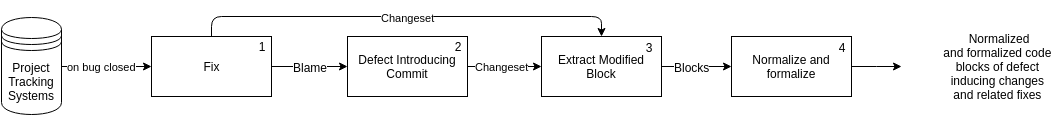
\includegraphics[width=\textwidth]{media/fix-approach.png}
    \caption{Managing events happening on project tracking systems to extract defect-introducing commits and commits that provided the fixes\label{fig:bianca1}}
\end{figure*}

\begin{figure*}
  \centering
    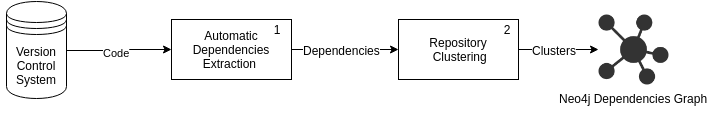
\includegraphics[width=0.7\textwidth]{media/cluster-approach}
    \caption{Clustering by dependency\label{fig:bianca3}}
\end{figure*}

\begin{figure*}
  \centering
    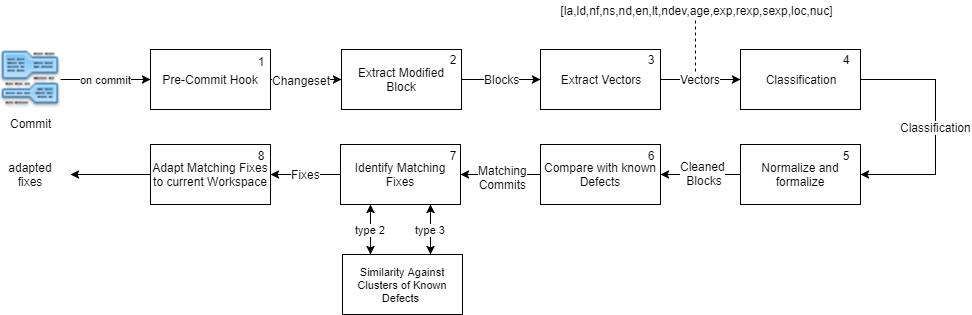
\includegraphics[width=\textwidth]{media/detect-approach}
    \caption{Classifying incoming commits and proposing fixes\label{fig:bianca2}}
\end{figure*}




These projects share many dependencies. We
clustered them based on their dependencies with the aim to improve the
accuracy of CLEVER. This clustering step is important in order to
identify faults that may exist due to dependencies, while enhancing the
quality of the proposed fixes.


In the second process (Figure \ref{fig:CLEVERT2}), CLEVER intercepts
incoming commits before they leave a developer's workstation using the
concept of pre-commit hooks. A pre-commit hook is a script that is
executed at commit-time and it is supported by most major code
versioning systems such as \emph{Git}. There are two types of hooks:
client-side and server-side. Client-side hooks are triggered by
operations such as committing and merging, whereas server-side hooks run
on network operations such as receiving pushed commits. These hooks can
be used for different purposes such as checking compliance with coding
rules, or the automatic execution of unit tests. A pre-commit hook runs
before a developer specifies a commit message.

Ubisoft's developers use pre-commit hooks for all sorts of reasons such
as identifying the tasks that are addressed by the commit at hand,
specifying the reviewers who will review the commit, and so on.
Implementing this part of CLEVER as a pre-commit hook is an important
step towards the integration of CLEVER with the workflow of developers
at Ubisoft. The developers do not have to download, install, and
understand additional tools in order to use CLEVER.

Once the commit is intercepted, we compute code and process metrics
associated with this commit. The selected metrics are discussed further
in Section \ref{sec:offline}. The result is a feature vector (Step 4)
that is used for classifying the commit as \emph{risky} or
\emph{non-risky}.

If the commit is classified as \emph{non-risky}, then the process stops,
and the commit can be transferred from the developer's workstation to
the central repository. \emph{Risky} commits, on the other hand, are
further analysed in order to reduce the number of false positives
(healthy commits that are detected as risky). We achieve this by first
extracting the code blocks that are modified by the developer and then
compare them to code blocks of known fault-introducing commits.

\subsection{Clustering Projects}\label{sec:clustering}

We cluster projects according to their dependencies. The rationale is
that projects that share dependencies are most likely to contain defects
caused by misuse of these dependencies. In this step, the project
dependencies are analysed and saved into a single NoSQL graph database
as shown in Figure \ref{fig:CLEVERT3}. A node corresponds to a project
that is connected to other projects on which it depends. Dependencies
can be \emph{external} or \emph{internal} depending on whether the
products are created in-house or supplied by a third-party. For
confidentiality reasons, we cannot reveal the name of the projects
involved in the project dependency graph. We show the 12 projects in
yellow color with their dependencies in blue color in Figure
\ref{fig:dep-graph}. In total, we discovered 405 distinct dependencies.
Dependencies can be internal (i.e.~library developed at Ubisoft) or
external (i.e.~library provided by third parties). The resulting
partitioning is shown in Figure \ref{fig:network-sample}.

\begin{figure}
  \centering
    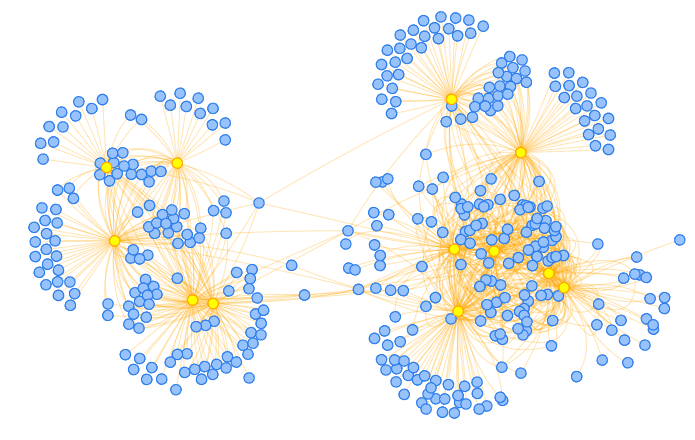
\includegraphics[width=0.5\textwidth]{media/network.png}
    \caption{Dependency Graph\label{fig:dep-graph}}
\end{figure}

At Ubisoft, dependencies are managed within the framework of a single
repository, which makes their automatic extraction possible. The
dependencies could also be automatically retrieved if the projects use a
dependency manager such as Maven.

\begin{figure*}
  \centering
    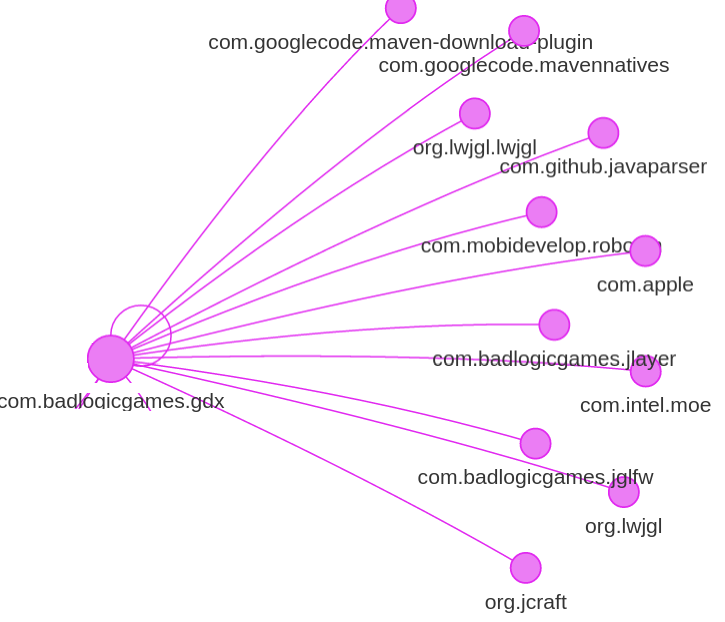
\includegraphics[width=0.60\textwidth]{media/network-sample.png}
    \caption{Simplified Dependency Graph for \texttt{com.badlogicgames.gdx}\label{fig:network-sample}}
\end{figure*}

Once the project dependency graph is extracted, we use a clustering
algorithm to partition the graph. To this end, we choose the
Girvan--Newman algorithm [10, 34], used to detect communities by
progressively removing edges from the original network. Instead of
trying to construct a measure that identifies the edges that are the
most central to communities, the Girvan--Newman algorithm focuses on
edges that are most likely ``between'' communities. This algorithm is
very effective at discovering community structure in both
computer-generated and real-world network data [34]. Other
clustering algorithms can also be used.

\subsection{Building a Database of Code Blocks of Defect-Commits and
Fix-Commits}\label{sec:offline}

To build our database of code blocks that are related to defect-commits
and fix-commits, we first need to identify the respective commits. Then,
we extract the relevant blocks of code from the commits.

\subsubsection{Extracting Commits:}\label{extracting-commits}

CLEVER listens to issue closing events happening on the project tracking
system used at Ubisoft. Every time an issue is closed, CLEVER retrieves
the commit that was used to fix the issue (the fix-commit) as well as
the one that introduced the defect (the defect-commit). To link
fix-commits and their related issues we implemented the well-known SZZ
algorithm presented by Kim et al. [23].

\subsubsection{Extracting Code Blocks:}\label{extracting-code-blocks}

Algorithm \ref{alg:extract} presents an overview of how to extract
blocks. This algorithm receives as arguments, the changesets and the
blocks that have been previously extracted. Then, Lines 1 to 5 show the
\(for\) loop that iterates over the changesets. For each changeset (Line
2), we extract the blocks by calling the
\(~extract\_blocks(Changeset~cs)\) function. In this function, we expand
our changeset to the left and to the right in order to have a complete
block.

\begin{algorithm}
 \KwData{$Changeset[]$ changesets\;
 $Block[]$ prior\_blocks\;
 }
 \KwResult{Up to date blocks of the systems}
 \For{$i \leftarrow 0$ \KwTo$size\_of~changesets$}{
    Block[] blocks $\leftarrow$ $extract\_blocks(changesets)$\;
    \For{$j \leftarrow 0$ \KwTo$size\_of~blocks$}{
       write $blocks[j]$\;
    }
 }

 \SetKwProg{myproc}{Function}{ $~extract\_blocks(Changeset~cs)$}{}
   \myproc{{}}{

   \uIf{$cs~is~unbalanced~right$}{$cs \leftarrow expand\_left(cs)$\;}

   \ElseIf{$cs~is~unbalanced~left$}{$cs \leftarrow expand\_right(cs)$\;}

   \nl\KwRet$txl\_extract\_blocks(cs)$\;
   }


 \caption{Overview of the Extract Blocks Operation\label{alg:extract}}
\end{algorithm}

As depicted by the diff below (not from Ubisoft), changesets contain
only the modified chunk of code and not necessarily complete blocks.

\begin{Shaded}
\begin{Highlighting}[]
\DataTypeTok{@@ -315,36 +315,6 @@}
\NormalTok{int initprocesstree_sysdep}
\NormalTok{(ProcessTree_T **reference) \{}
    \NormalTok{mach_port_deallocate(mytask,}
      \NormalTok{task);}
\NormalTok{\}}
\NormalTok{\}}
\StringTok{- if (task_for_pid(mytask, pt[i].pid,}
\StringTok{-  &task) == KERN_SUCCESS) \{}
\StringTok{-   mach_msg_type_number_t   count;}
\StringTok{-   task_basic_info_data_t   taskinfo;}
\end{Highlighting}
\end{Shaded}

Therefore, we need to expand the changeset to the left (or right) to
have syntactically correct blocks. We do so by checking the block's
beginning and ending with parentheses algorithms [3].

\subsection{Building a Metric-Based Model}\label{sec:metric-based}

We adapted Commit-guru [38] for building the metric-based model.
Commit-guru uses a list of keywords proposed by Hindle \emph{et al.}
[14] to classify commit in terms of \emph{maintenance},
\emph{feature} or \emph{fix}. Then, it uses the SZZ algorithm to find
the defect-commit linked to the fix-commit. For each defect-commit,
Commit-guru computes the following code metrics: \emph{la} (lines
added), \emph{ld} (lines deleted), \emph{nf} (number of modified files),
\emph{ns} (number of modified subsystems), \emph{nd} (number of modified
directories), \emph{en} (distriubtion of modified code across each
file), \emph{lt} (lines of code in each file (sum) before the commit),
\emph{ndev} (the number of developers that modifed the files in a
commit), \emph{age} (the average time interval between the last and
current change), \emph{exp} (number of changes previously made by the
author ), \emph{rexp} (experience weighted by age of files (1 / (n +
1))), \emph{sexp} (previous changes made by the author in the same
subsystem), \emph{loc} (total number of modified LOC across all files),
\emph{nuc} (number of unique changes to the files). Then, a statistical
model is built using the metric values of the defect-commits. Using
linear regression, Commit-guru is able to predict whether incoming
commits are \emph{risky} or not.

We had to modify Commit-guru to fit the context of this study. First, we
used information found in Ubisoft's internal project tracking system to
classify the purpose of a commit (i.e., \emph{maintenance},
\emph{feature} or \emph{fix}). In other words, CLEVER only classifies a
commit as a defect-commit if it is the root cause of a fix linked to a
crash or a bug in the internal project tracking system. Using internal
pre-commit hooks, Ubisoft developers must link every commit to a given
task \#ID. If the task \#ID entered by the developer matches a bug or
crash report within the project tracking system, then we perform the SCM
blame/annotate function on all the modified lines of code for their
corresponding files on the fix-commit's parents. This returns the
commits that previously modified these lines of code and are flagged as
defect-commits. Another modification consists of the actual
classification algorithm. We did not use linear regression but instead
the random forest algorithm [45, 46]. The random forest algorithm
turned out to be more effective as described in Section
\ref{sec:result}. Finally, we had to rewrite Commit-guru in GoLang for
performance and internal reasons.

\subsection{Comparing Code Blocks}\label{sec:online}

Each time a developer makes a commit, CLEVER intercepts it using a
pre-commit hook and classifies it as \emph{risky} or not. If the commit
is classified as \emph{risky} by the metric-based classifier, then, we
extract the corresponding code block (in a similar way as in the
previous phase), and compare it to the code blocks of historical
defect-commits. If there is a match, then the new commit is deemed to be
risky. A threshold \(\alpha\) is used to assess the extent beyond which
two commits are considered similar.

To compare the extracted blocks to the ones in the database, we resort
to clone detection techniques, more specifically, text-based clone
detection techniques. This is because lexical and syntactic analysis
approaches (alternatives to text-based comparisons) would require a
complete program to work, i.e., a program that compiles. In the
relatively wide-range of tools and techniques that exist to detect
clones by considering code as text [8, 16, 17, 29, 30, 47], we chose
the NICAD clone detector because it is freely available and has shown to
perform well [6].

NICAD can detect Type 1, 2 and 3 software clones [21]. Type 1 clones
are copy-pasted blocks of code that only differ from each other in terms
of non-code artifacts such as indentation, whitespaces, comments and so
on. Type 2 clones are blocks of code that are syntactically identical
except literals, identifiers, and types that can be modified. Also, Type
2 clones share the particularities of Type 1 about indentation,
whitespaces, and comments. Type 3 clones are similar to Type 2 clones in
terms of modification of literals, identifiers, types, indentation,
whitespaces, and comments but also contain added or deleted code
statements.

The problem with the current implementation of NICAD is that it only
considers complete Java, C\#, and C files. We improved NICAD to process
blocks that come from commit-diffs. This is because the current version
of NICAD can only process syntactically correct code and commit-diffs
are, by definition, snippets that represent modified regions of a given
set of files.

By reusing NICAD, CLEVER can detect Types 3 software clones [21].
Type 3 clones can contain added or deleted code statements, which make
them suitable for comparing commit code blocks. In addition, NICAD uses
a pretty-printing strategy from where statements are broken down into
several lines [40]. This functionality allowed us to detect Segments
1 and 2 as a clone pair, as shown by Table \ref{tab:pretty-printing},
because only the initialization of \(i\) changed. This specific example
would not have been marked as a clone by other tools we tested such as
Duploc [8].

\begin{table*}[]
\centering
\caption{Pretty-Printing Example}
\label{tab:pretty-printing}
\resizebox{0.5\textwidth}{!}{%
\begin{tabular}{l|l|l|l|l|l}
\hline
Segment 1          & Segment 2          & Segment 3           & S1 \& S2 & S1 \& S3 & S2 \& S3 \\ \hline \hline
for (              & for (              & for (               & 1        & 1        & 1        \\
i = 0;             & i = 1;             & j = 2;              & 0        & 0        & 0        \\
i \textgreater 10; & i \textgreater 10; & j \textgreater 100; & 1        & 0        & 0        \\ 
i++)               & i++)               & j++)                & 1        & 0        & 0        \\ \hline \hline
\multicolumn{3}{c|}{Total Matches}                            & 3        & 1        & 1        \\ \hline
\multicolumn{3}{c|}{Total Mismatches}                         & 1        & 3        & 3 \\ \hline

\end{tabular}
}
\end{table*}

The extracted, pretty-printed, normalized filtered blocks are marked as
potential clones using a Longest Common Subsequence (LCS) algorithm
[15]. Then, a percentage of unique statements can be computed and,
given the threshold \(\alpha\), the blocks are marked as clones.

\subsection{Classifying Incoming
Commits}\label{classifying-incoming-commits}

As discussed in Section \ref{sec:metric-based}, a new commit goes
through the metric-based model first (Steps 1 to 4). If the commit is
classified as \emph{non-risky}, we simply let it through, and we stop
the process. If the commit is classified as \emph{risky}, however, we
continue the process with Steps 5 to 8 in our approach.

One may wonder why we needed to have a metric-based model in the first
place. We could have resorted to clone detection as the main mechanism.
The main reason for having the metric-based model is efficiency. If each
commit had to be analysed against all known signatures using code clone
similarity, then, it would have made CLEVER more time consuming. We
estimate that, in an average workday, if all commits had to be compared
against all signatures on the same cluster we used for our experiments
it would take around 25 minutes to process a commit. In comparison, it
takes, in average, 3.75 seconds with the current approach.

\subsection{Proposing Fixes}\label{proposing-fixes}

An important aspect in the design of CLEVER is the ability to provide
guidance to developers on how to improve risky commits. We achieve this
by extracting from the database the fix-commit corresponding to the top
1 matching defect-commits and present it to the developer. We believe
that this makes CLEVER a practical approach. Developers can understand
why a given modification has been reported as risky by looking at code
instead of simple metrics as in the case of the studies reported in
[19, 38].

Finally, using the fixes of past defects, we can provide a solution, in
the form of a contextualised diff, to developers. A contextualised diff
is a diff that is modified to match the current workspace of the
developer regarding variable types and names. In Step 8 of Figure 3, we
adapt the matching fixes to the actual context of the developer by
modifying indentation depth and variable name in an effort to reduce
context switching. We believe that this would make it easier for
developers to understand the proposed fixes and see if it applies in
their situation.

All the proposed fixes will come from projects in the same cluster as
the project where the \emph{risky} commit is. Thus, developers have
access to fixes that should be easier to understand as they come from
projects similar to theirs inside the company.

\section{Case Study Setup}\label{sec:exp}

In this section, we present the setup of our case study in terms of
repository selection, dependency analysis, comparison process and
evaluation measures.

\subsection{Project Repository Selection}\label{sec:rep}

In collaboration with Ubisoft developers, we selected 12 major software
projects (i.e., systems) developed at Ubisoft to evaluate the
effectiveness of CLEVER. These systems continue to be actively
maintained by thousands of developers. Ubisoft projects are organized by
game engines. A game engine can be used in the development of many
high-budget games. The projects selected for this case study are related
to the same game engine. For confidentiality and security reasons,
neither the names nor the characteristics of these projects are
provided. We can however disclose that the size of these systems
altogether consists of millions of lines of code.

\subsection{Project Dependency Analysis}\label{sec:dependencies}

Figure \ref{fig:dep-graph} shows the project dependency graph. As shown
in Figure \ref{fig:dep-graph}, these projects are highly interconnected.
A review of each cluster shows that this partitioning divides projects
in terms of their high-level functionalities. For example, one cluster
is related to a particular given family of video games, whereas the
other cluster refers to another family. We showed this partitioning to
11 experienced software developers and ask them to validate it. They all
agreed that the results of this automatic clustering are accurate and
reflects well the various project groups of the company. The clusters
are used for decreasing the rate of false positive. In addition, fixes
mined across projects but within the cluster are qualitative as shown in
our experiments.

\subsection{Building a Database of Defect-Commits and
Fix-Commits}\label{sub:golden}

To build the database that we can use to assess the performance of
CLEVER, we use the same process as discussed in Section
\ref{sec:offline}. We retrieve the full history of each project and
label commits as defect-commits if they appear to be linked to a closed
issue using the SZZ algorithm [23]. This baseline is used to compute
the precision and recall of CLEVER. Each time CLEVER classifies a commit
as \emph{risky}; we can check if the \emph{risky} commit is in the
database of defect-introducing commits. The same evaluation process is
used by related studies [1, 9, 20, 25, 28].

\subsection{Process of Comparing New Commits}\label{sec:newcommits}

Because our approach relies on commit pre-hooks to detect risky commits,
we had to find a way to \emph{replay} past commits. To do so, we
\emph{cloned} our test subjects, and then created a new branch called
\emph{CLEVER}. When created, this branch is reinitialized at the initial
state of the project (the first commit), and each commit can be replayed
as they have originally been. For each commit, we store the time taken
for \emph{CLEVER} to run, the number of detected clone pairs, and the
commits that match the current commit. As an example, suppose that we
have three commits from two projects. At time \(t_1\), commit \(c_1\) in
project \(p_1\) introduces a defect. The defect is experienced by a user
that reports it via an issue \(i_1\) at \(t_2\). A developer fixes the
defect introduced by \(c_1\) in commit \(c_2\) and closes \(i_1\) at
\(t_3\). From \(t_3\) we know that \(c_1\) introduced a defect using the
process described in Section \ref{sub:golden}. If at \(t_4\), \(c_3\) is
pushed to \(p_2\) and classified by the metric-based classifier as
\emph{risky}, we extract \(c_3\) blocks and compare them with the ones
of \(c_1\). If \(c3\) and \(c1\) are a match after preprocessing,
pretty-printing and formatting, then \(c_3\) is classified as
\emph{risky} by CLEVER and \(c_2\) is proposed to the developer as a
potential solution for the defect introduced in \(c_3\).

\subsection{Evaluation Measures}\label{evaluation-measures}

Similar to prior work (e.g., [20, 43]), we used precision, recall,
and F\(_1\)-measure to evaluate our approach. They are computed using TP
(true positives), FP (false positives), FN (false negatives), which are
defined as follows:

\begin{itemize}
\tightlist
\item
  TP is the number of defect-commits that were properly classified by
  CLEVER
\item
  FP is the number of healthy commits that were classified by CLEVER as
  risky
\item
  FN is the number of defect introducing-commits that were not detected
  by CLEVER
\item
  Precision: TP / (TP + FP)
\item
  Recall: TP / (TP + FN)
\item
  F\(_1\)-measure:
  \(2 \times (precision \times recall)/(precision+recall)\)
\end{itemize}

It is worth mentioning that, in the case of defect prevention, false
positives can be hard to identify as the defects could be in the code
but not yet reported through a bug report (or issue). To address this,
we did not include the last six months of history. Following similar
studies [4, 18, 38, 41], if a defect is not reported within six
months then it is not considered.

\section{Case Study Results}\label{sec:result}

In this section, we show the effectiveness of CLEVER in detecting risky
commits using a combination of metric-based models and clone detection.
The main research question addressed by this case study is: \emph{Can we
detect risky commits by combining metrics and code comparison within and
across related Ubisoft projects, and if so, what would be the accuracy?}

The experiments took nearly two months using a cluster of six 12 3.6 Ghz
cores with 32GB of RAM each. The most time consuming part of the
experiment consists of building the baseline as each commit must be
analysed with the SZZ algorithm. Once the baseline was established, the
model built, it took, on average, 3.75 seconds to analyse an incoming
commit on our cluster.

In the following subsections, we provide insights on the performance of
CLEVER by comparing it to Commit-guru [38] alone, i.e., an approach
that relies only on metric-based models. We chose Commit-guru because it
has been shown to outperform other techniques (e.g., [19, 25]).
Commit-guru is also open source and easy to use.

\subsection{Performance of CLEVER}\label{performance-of-clever}

When applied to 12 Ubisoft projects, CLEVER detects risky commits with
an average precision, recall, and F1-measure of 79.10\%, a 65.61\%, and
71.72\% respectively. For clone detection, we used a threshold of 30\% .
This is because Roy \emph{et al.} [39] showed through empirical
studies that using NICAD with a threshold of around 30\%, the default
setting, provides good results for the detection of Type 3 clones. When
applied to the same projects, Commit-guru achieves an average precision,
recall, and F1-measure of 66.71\%, 63.01\% and 64.80\%, respectively.

We can see that with the second phase of CLEVER (clone detection) there
is considerable reduction in the number of false positives (precision of
79.10\% for CLEVER compared to 66.71\% for Commit-guru) while achieving
similar recall (65.61\% for CLEVER compared to 63.01\% for Commit-guru).

\begin{table*}[]
\centering
\caption{Workshop results}
\label{tab:Workshop}
\begin{tabular}{c|c|c|c|c|c|c|c|c|c|c|c|c}
   & F1        & F2 & F3        & F4        & F5 & F6        & F7 & F8        & F9 & F10       & F11       & F12 \\ \hline
P1 & Accepted & Rejected   & Accepted & Accepted & Unsure  & Accepted & Unsure  & Rejected          & Rejected   & Accepted & Accepted & Unsure   \\
P2 & Accepted & Rejected   & Accepted & Unsure         & Unsure  & Accepted & Unsure  & Rejected          & Rejected   & Accepted & Accepted & Unsure   \\
P3 & Accepted & Rejected   & Accepted & Unsure         & Unsure  & Accepted & Unsure  & Rejected          & Rejected   & Accepted & Accepted & Unsure   \\
P4 & Accepted & Rejected   & Accepted & Unsure         & Unsure  & Accepted & Unsure  & Accepted & Rejected   & Accepted & Accepted & Unsure   \\
P5 & Accepted & Rejected   & Accepted & Accepted & Unsure  & Accepted & Unsure  & Rejected          & Rejected   & Accepted & Accepted & Unsure   \\
P6 & Accepted & Rejected   & Accepted & Unsure         & Unsure  & Accepted & Unsure  & Accepted & Rejected   & Accepted & Accepted & Unsure   \\ \hline
\end{tabular}
\end{table*}

\subsection{Analysis of the Quality of the Fixes Proposed by
CLEVER}\label{analysis-of-the-quality-of-the-fixes-proposed-by-clever}

In order to validate the quality of the fixes proposed by CLEVER, we
conducted an internal workshop where we invited a number of people from
Ubisoft development team. The workshop was attended by six participants:
two software architects, two developers, one technical lead, and one IT
project manager. The participants have many years of experience at
Ubisoft.

The participants were asked to review 12 randomly selected fixes that
were proposed by CLEVER. These fixes are related to one system in which
the participants have excellent knowledge. We presented them with the
original buggy commits, the original fixes for these commits, and the
fixes that were automatically extracted by CLEVER. We asked them the
following question \emph{``Is the proposed fix applicable in the given
situation?''} for each fix.

The review session took around 50 minutes. This does not include the
time it took to explain the objective of the session, the setup, the
collection of their feedback, etc.

We asked the participants to rank each fix proposed by CLEVER using this
scheme:

\begin{itemize}
\tightlist
\item
  Fix Accepted: The participant found the fix proposed by CLEVER
  applicable to the risky commit.
\item
  Unsure: In this situation, the participant is unsure about the
  relevance of the fix. There might be a need for more information to
  arrive to a verdict.
\item
  Fix Rejected: The participant found the fix is not applicable to the
  risky commit.
\end{itemize}

Table \ref{tab:Workshop} shows answers of the participants. The columns
refer to the fixes proposed by CLEVER, whereas the rows refer to the
participants that we denote using P1, P2, \ldots{}, P6. As we can see
from the table, 41.6\% of the proposed fixes (F1, F3, F6, F10 and F12)
have been accepted by all participants, while 25\% have been accepted by
at least one member (F4, F8, F11). We analysed the fixes that were
rejected by some or all participants to understand the reasons.

\(F2\) was rejected by our participants because the region of the commit
that triggered a match is a generated code. Although this generated code
was pushed into the repositories as part of bug fixing commit, the root
cause of the bug lies in the code generator itself. Our proposed fix
suggests to update the generated code. Because the proposed fix did not
apply directly to the bug and the question we ask our reviewers was
\emph{``Is the proposed fix applicable in the given situation?''} they
rejected it. In this occurrence, the proposed fix was not applicable.

\(F4\) was accepted by two reviewers and marked as unsure by the other
participants. We believe that this was due the lack of context
surrounding the proposed fix. The participants were unable to determine
if the fix was applicable or not without knowing what the original
intent of the buggy commit was. In our review session, we only provided
the reviewers with the regions of the commits that matched existing
commits and not the full commit. Full commits can be quite lengthy as
they can contain asset descriptions and generated code, in addition to
the actual code. In this occurrence, the full context of the commit
might have helped our reviewers to decide if \(F4\) was applicable or
not. \(F5\) and \(F7\) were classified as unsure by all our participants
for the same reasons.

\(F8\) was rejected by four of participants and accepted by two. The
participants argued that the proposed fix was more a refactoring
opportunity than an actual fix.

\(F12\) was marked as unsure by all the reviewers because the code had
to do with a subsystem that is maintained by another team and the
participants felt that it was out of scope of this session.

After the session, we asked the participants two additional questions:
\emph{Will you use CLEVER in the future?} and \emph{What aspects of
CLEVER need to be improved?}

All the participants answered the first question favourably. They also
proposed to embed CLEVER with Ubisoft's quality assurance tool suite.
The participants reported that the most useful aspects of CLEVER are:

\begin{itemize}
\tightlist
\item
  Ability to leverage many years of historical data of inter-related
  projects, hence allowing development teams to share their experiences
  in fixing bugs.
\item
  Easy integration of CLEVER into developers' work flow based on the
  tool's ability to operate at commit-time.\\
\item
  Precision and recall of the tool (79\% and 65\% respectively)
  demonstrating CLEVER's capabilities to catch many defects that would
  otherwise end up in the code repository. For the second question, the
  participants proposed to add a feedback loop to CLEVER where the input
  of software developers is taken into account during classification.
  The objective is to reduce the number of false negatives (risky
  commits that are flagged as non-risky) and false positives (non-risky
  commits that are flagged as risky). The feedback loop mechanism would
  work as follows: When a commit is misclassified by the tool, the
  software developer can choose to ignore CLEVER's recommendation and
  report the misclassified commit. If the fix proposition is not used,
  then, we would give that particular pattern less strength over other
  patterns automatically.
\end{itemize}

We do not need manual input from the user because CLEVER knows the state
of the commit before the recommendation and after. If both versions are
identical then we can mark the recommendation as not helpful. This way,
we can also compensate for human error (i.e., a developer rejecting
CLEVER recommendation when the commit was indeed introducing a defect.
We would know this by using the same processes that allowed us to build
our database of defect-commits as described in Section
\ref{sec:offline}. This feature is currently under development.

It is worth noting that Ubisoft developers who participated to this
study did not think that CLEVER fixes that were deemed irrelevant were a
barrier to the deployment of CLEVER. In their point of view, the
performance of CLEVER in terms of classification should make a
significant impact as suspicious commits will receive extended reviews
and/or further investigations.

We are also investigating the use of adaptive learning techniques to
improve the classification mechanism of CLEVER. In addition to this, the
participants discussed the limitation of CLEVER as to its inability to
deal with automatically generated code. We are currently working with
Ubisoft's developers to address this limitation.

\subsection{Deployment of CLEVER at
Ubisoft}\label{deployment-of-clever-at-ubisoft}

CLEVER is now beginning to be rolled out at Ubisoft. It will be made
available to thousands of developers across various divisions. Our
research team provided on-site training of this new tool. In addition,
Ubisoft developed an instructional video to support the launch of CLEVER
and raise awareness about the tool. Our research team is currently
monitoring the use of CLEVER at Ubisoft to evaluate its adoption (usage,
barriers, etc.).

\section{Discussion}\label{sec:threats}

In this section, we share the lessons learned, discuss the limitations
of CLEVER, and present threats to validity of our study.

\subsection{Lessons Learned}\label{lessons-learned}

\subsubsection{Understanding the industrial
context:}\label{understanding-the-industrial-context}

Throughout the design of CLEVER, we made many design decisions that were
triggered by the discussions we had with Ubisoft developers. Some of the
key decisions that we made included having CLEVER operate on clusters of
inter-related systems and combining metric-based and code matching
techniques into a two-phase approach. These decisions were not only
critical in obtaining an improved accuracy, but also in proposing
effective fixes that guide developers. From our interactions with
Ubisoft developers, it was also important for us to come up with a
solution that integrates well with the workflow of Ubisoft developers.
This motivated the use of commit-time and the integration of CLEVER with
Ubisoft version control systems. The key lesson here is the importance
of understanding the industrial context by working with the company's
development teams. This collaboration is also an enabler for the
adoption of tools, developed in the context of research projects.

\subsubsection{Leveraging an iterative
process:}\label{leveraging-an-iterative-process}

Throughout this research project, we followed an iterative and
incremental process. The results of each iteration were presented to
Ubisoft developers for feedback. Adjustments were made as needed, before
the subsequent iteration started. This process was not only helpful in
keeping the project on track, but also in producing ``quick wins'' as a
way of showing practical results from each iteration. Examples of such
``quick wins'' include the creation of the defect introduction landscape
at Ubisoft in terms of number defects, time to fix defects and time to
discover defects organization wide. In addition, the computed clusters
of similar projects turned out to be useful for upper management in
order to organize collaborations between teams belonging to different
projects.

\subsubsection{Communicating
effectively:}\label{communicating-effectively}

During the development of CLEVER, we needed to constantly communicate
the steps of our research to developers and project owners. It was
important to adopt a communication strategy suitable to each
stakeholder. For example, in our meetings with management, we focused
more on the ability of CLEVER to improve code quality and reduce
maintenance costs instead of the technical details of the proposed
approach. Developers, on the other hand, were interested in the
potential of CLEVER and its integration with their work environment.

\subsubsection{Underestimating the time needed for full deployment of
CLEVER:}\label{underestimating-the-time-needed-for-full-deployment-of-clever}

Part of our mandate was to develop a working tool. It took a tremendous
amount of time and effort to bring CLEVER to a production level and
integrate it with Ubisoft tool suite. Most of the work involved was pure
engineering work that went beyond research. We recognize that we
underestimated the complexity of this task. Examples of deliverables we
had to produce include automating the acquisition of new commits,
presenting the recommendations to the developers, building grammars for
various programming languages, creating APIs that interact with any
types of client systems, authentication, and authorization of end-users,
etc. Overall, the machine learning code represents less than 5\% of our
code base. The lesson here is to manage expectations and to better
estimate the project time and effort from an end to end perspective, and
not only the research part.

\subsection{Limitations}\label{limitations}

We identified two main limitations of our approach, CLEVER, which
require further studies.

CLEVER is designed to work on multiple related systems. Applying CLEVER
to a single system will most likely be less effective. The two-phase
classification process of CLEVER would be hindered by the fact that it
is unlikely to have a large number of similar bugs within the same
system. For single systems, we recommend the use of metric-based models.
A metric-based solution, however, may turn to be ineffective when
applied across systems because of the difficulty associated with
identifying common thresholds that are applicable to a wide range of
systems.

The second limitation we identified has to do with the fact that CLEVER
is designed to work with Ubisoft systems. Ubisoft uses C\#, C, C++, Java
and other internally developed languages. It is however common to have
other languages used in an environment with many inter-related systems.
We intend to extend CLEVER to process commits from other languages as
well.

\subsection{Threats to Validity}\label{threats-to-validity}

The selection of target systems is one of the common threats to validity
for approaches aiming to improve the analysis of software systems. It is
possible that the selected programs share common properties that we are
not aware of and therefore, invalidate our results. Because of the
industrial nature of this study, we had to work with the systems
developed by the company.

The programs we used in this study are all based on the C\#, C, C++ and
Java programming languages. This can limit the generalization of the
results to projects written in other languages, especially that the main
component of CLEVER is based on code clone matching.

Finally, part of the analysis of the CLEVER proposed fixes that we did
was based on manual comparisons of the CLEVER fixes with those proposed
by developers with a focus group composed of experienced engineers and
software architects. Although, we exercised great care in analysing all
the fixes, we may have misunderstood some aspects of the commits.

In conclusion, internal and external validity have both been minimized
by choosing a set of 12 different systems, using input data that can be
found in any programming languages and version systems (commits and
changesets).

\section{Conclusion}\label{sec:conclusion}

In this paper, we presented CLEVER (Combining Levels of Bug Prevention
and Resolution Techniques), an approach that detects risky commits
(i.e., a commit that is likely to introduce a bug) with an average of
79.10\% precision and a 65.61\% recall. CLEVER combines code metrics,
clone detection techniques, and project dependency analysis to detect
risky commits within and across projects. CLEVER operates at
commit-time, i.e., before the commits reach the central code repository.
Also, because it relies on code comparison, CLEVER does not only detect
risky commits but also makes recommendations to developers on how to fix
them. We believe that this makes CLEVER a practical approach for
preventing bugs and proposing corrective measures that integrate well
with the developer's workflow through the commit mechanism. CLEVER is
still in its infancy and we expect it to be available this year to
thousands of developers.

As future work, we want to build a feedback loop between the users and
the clusters of known buggy commits and their fixes. If a fix is never
used by the end-users, then we could remove it from the clusters and
improve our accuracy. We also intend to improve CLEVER to deal with
generated code. Moreover, we will investigate how to improve the fixes
proposed by CLEVER to add contextual information to help developers
better assess the applicability of the fixes.

\section{Reproduction Package}\label{reproduction-package}

For security and confidentiality reasons we cannot provide a
reproduction package that will inevitably involve Ubisoft's copyrighted
source code. However, the CLEVER source code is in the process of being
open-sourced and will be soon available at
https://github.com/ubisoftinc.

\begin{acks}
We are thankful to the software development team at  Ubisoft for their participations to the study and their assessment of the effectiveness of CLEVER.
We are also thankful to NSERC (Natural Sciences and Engineering Research Concil of Canada) which financed part of this research.
\end{acks}

\section*{References}

\setlength{\parindent}{0pt} \setlength{\parskip}{0.5em}



[1] Bhattacharya, P. and Neamtiu, I. 2011. Bug-fix time prediction
models: can we do better? \emph{Proceeding of the international
conference on mining software repositories} (New York, New York, USA,
May 2011), 207--210.


[2] Briand, L. et al. 1999. A unified framework for coupling
measurement in object-oriented systems. \emph{IEEE Transactions on
Software Engineering}. 25, 1 (1999), 91--121.
DOI:\url{https://doi.org/10.1109/32.748920}.


[3] Bultena, B. and Ruskey, F. 1998. An Eades-McKay algorithm for
well-formed parentheses strings. \emph{Information Processing Letters}.
68, 5 (1998), 255--259.


[4] Chen, T.-h. et al. 2014. An Empirical Study of Dormant Bugs
Categories and Subject Descriptors. \emph{Proceedings of the
international conference on mining software repository} (2014), 82--91.


[5] Chidamber, S. and Kemerer, C. 1994. A metrics suite for object
oriented design. \emph{IEEE Transactions on Software Engineering}. 20, 6
(Jun. 1994), 476--493. DOI:\url{https://doi.org/10.1109/32.295895}.


[6] Cordy, J.R. and Roy, C.K. 2011. The NiCad Clone Detector.
\emph{Proceedings of the international conference on program
comprehension} (Jun. 2011), 219--220.


[7] Dallmeier, V. et al. 2009. Generating Fixes from Object Behavior
Anomalies. \emph{Proceedings of the international conference on
automated software engineering} (2009), 550--554.


[8] Ducasse, S. et al. 1999. A Language Independent Approach for
Detecting Duplicated Code. \emph{Proceedings of the international
conference on software maintenance} (1999), 109--118.


[9] El Emam, K. et al. 2001. The prediction of faulty classes using
object-oriented design metrics. \emph{Journal of Systems and Software}.
56, 1 (Feb. 2001), 63--75.
DOI:\url{https://doi.org/10.1016/S0164-1212(00)00086-8}.


[10] Girvan, M. and Newman, M.E.J. 2002. Community structure in
social and biological networks. \emph{Proceedings of the National
Academy of Sciences}. 99, 12 (Jun. 2002), 7821--7826.
DOI:\url{https://doi.org/10.1073/pnas.122653799}.


[11] Gyimothy, T. et al. 2005. Empirical validation of
object-oriented metrics on open source software for fault prediction.
\emph{IEEE Transactions on Software Engineering}. 31, 10 (Oct. 2005),
897--910. DOI:\url{https://doi.org/10.1109/TSE.2005.112}.


[12] Hassan, A. and Holt, R. 2005. The top ten list: dynamic fault
prediction. \emph{Proceedings of the international conference on
software maintenance} (2005), 263--272.


[13] Hassan, A.E. 2009. Predicting faults using the complexity of
code changes. \emph{Proceedings of the international conference on
software engineering} (May 2009), 78--88.


[14] Hindle, A. et al. 2008. What do large commits tell us?: a
taxonomical study of large commits. \emph{Proceedings of the
international workshop on mining software repositories} (New York, New
York, USA, 2008), 99--108.


[15] Hunt, J.W. and Szymanski, T.G. 1977. A fast algorithm for
computing longest common subsequences. \emph{Communications of the ACM}.
20, 5 (May 1977), 350--353.
DOI:\url{https://doi.org/10.1145/359581.359603}.


[16] Johnson, J.H. 1993. Identifying redundancy in source code using
fingerprints. \emph{Proceedings of the conference of the centre for
advanced studies on collaborative research} (Oct. 1993), 171--183.


[17] Johnson, J.H. 1994. Visualizing textual redundancy in legacy
source. \emph{Proceedings of the conference of the centre for advanced
studies on collaborative research} (Oct. 1994), 32.


[18] Kamei, Y. et al. 2013. A large-scale empirical study of
just-in-time quality assurance. \emph{IEEE Transactions on Software
Engineering}. 39, 6 (Jun. 2013), 757--773.
DOI:\url{https://doi.org/10.1109/TSE.2012.70}.


[19] Kamei, Y. et al. 2013. A large-scale empirical study of
just-in-time quality assurance. \emph{IEEE Transactions on Software
Engineering}. 39, 6 (Jun. 2013), 757--773.
DOI:\url{https://doi.org/10.1109/TSE.2012.70}.


[20] Kamei, Y. et al. 2013. A large-scale empirical study of
just-in-time quality assurance. \emph{IEEE Transactions on Software
Engineering}. 39, 6 (Jun. 2013), 757--773.
DOI:\url{https://doi.org/10.1109/TSE.2012.70}.


[21] Kapser, C. and Godfrey, M.W. 2003. Toward a Taxonomy of Clones
in Source Code: A Case Study. \emph{International workshop on evolution
of large scale industrial software architectures} (2003), 67--78.


[22] Kim, D. et al. 2013. Automatic patch generation learned from
human-written patches. \emph{Proceedings of the international conference
on software engineering} (May 2013), 802--811.


[23] Kim, S. et al. 2006. Automatic Identification of
Bug-Introducing Changes. \emph{Proceedings of the international
conference on automated software engineering} (2006), 81--90.


[24] Kim, S. et al. 2007. Predicting Faults from Cached History.
\emph{Proceedings of the international conference on software
engineering} (May 2007), 489--498.


[25] Kpodjedo, S. et al. 2010. Design evolution metrics for defect
prediction in object oriented systems. \emph{Empirical Software
Engineering}. 16, 1 (Dec. 2010), 141--175.
DOI:\url{https://doi.org/10.1007/s10664-010-9151-7}.


[26] Le Goues, C. et al. 2012. A systematic study of automated
program repair: Fixing 55 out of 105 bugs for \$8 each.
\emph{Proceedings of the international conference on software
engineering} (2012), 3--13.


[27] Le, X.-B.D. et al. 2015. Should fixing these failures be
delegated to automated program repair? \emph{Proceedings of the
international symposium on software reliability engineering} (2015),
427--437.


[28] Lee, T. et al. 2011. Micro interaction metrics for defect
prediction. \emph{Proceedings of the european conference on foundations
of software engineering} (New York, New York, USA, 2011), 311--231.


[29] Manber, U. 1994. Finding similar files in a large file system.
\emph{Proceedings of the usenix winter} (Jan. 1994), 1--10.


[30] Marcus, A. and Maletic, J. 2001. Identification of high-level
concept clones in source code. \emph{Proceedings international
conference on automated software engineering} (2001), 107--114.


[31] Nagappan, N. and Ball, T. 2005. Static analysis tools as early
indicators of pre-release defect density. \emph{Proceedings of the
international conference on software engineering} (New York, New York,
USA, May 2005), 580--586.


[32] Nagappan, N. and Ball, T. 2005. Use of relative code churn
measures to predict system defect density. \emph{Proceedings of the
international conference on software engineering} (2005), 284--292.


[33] Nagappan, N. et al. 2006. Mining metrics to predict component
failures. \emph{Proceeding of the international conference on software
engineering} (New York, New York, USA, May 2006), 452--461.


[34] Newman, M.E.J. and Girvan, M. 2004. Finding and evaluating
community structure in networks. \emph{Physical Review E}. 69, 2 (Feb.
2004), 026113. DOI:\url{https://doi.org/10.1103/PhysRevE.69.026113}.


[35] Ostrand, T. et al. 2005. Predicting the location and number of
faults in large software systems. \emph{IEEE Transactions on Software
Engineering}. 31, 4 (Apr. 2005), 340--355.
DOI:\url{https://doi.org/10.1109/TSE.2005.49}.


[36] Pan, K. et al. 2008. Toward an understanding of bug fix
patterns. \emph{Empirical Software Engineering}. 14, 3 (Aug. 2008),
286--315. DOI:\url{https://doi.org/10.1007/s10664-008-9077-5}.


[37] Rahman, F. and Devanbu, P. 2013. How, and why, process metrics
are better. \emph{Proceedings of the international conference on
software engineering} (2013), 432--441.


[38] Rosen, C. et al. 2015. Commit guru: analytics and risk
prediction of software commits. \emph{Proceedings of the joint meeting
on foundations of software engineering} (New York, New York, USA, Aug.
2015), 966--969.


[39] Roy, C. and Cordy, J. 2008. NICAD: Accurate Detection of
Near-Miss Intentional Clones Using Flexible Pretty-Printing and Code
Normalization. \emph{2008 16th iEEE international conference on program
comprehension} (Jun. 2008), 172--181.


[40] Roy, C.K. 2009. \emph{Detection and Analysis of Near-Miss
Software Clones}. Queen's University.


[41] Shivaji, S. et al. 2013. Reducing Features to Improve Code
Change-Based Bug Prediction. \emph{IEEE Transactions on Software
Engineering}. 39, 4 (2013), 552--569.


[42] Subramanyam, R. and Krishnan, M. 2003. Empirical analysis of CK
metrics for object-oriented design complexity: implications for software
defects. \emph{IEEE Transactions on Software Engineering}. 29, 4 (Apr.
2003), 297--310. DOI:\url{https://doi.org/10.1109/TSE.2003.1191795}.


[43] Sunghun Kim, S. et al. 2008. Classifying Software Changes:
Clean or Buggy? \emph{IEEE Transactions on Software Engineering}. 34, 2
(Mar. 2008), 181--196. DOI:\url{https://doi.org/10.1109/TSE.2007.70773}.


[44] Tao, Y. et al. 2014. Automatically generated patches as
debugging aids: a human study. \emph{Proceedings of the international
symposium on foundations of software engineering} (2014), 64--74.


[45] Tin Kam Ho 1995. Random decision forests. \emph{Proceedings of
the international conference on document analysis and recognition}
(1995), 278--282.


[46] Tin Kam Ho 1998. The random subspace method for constructing
decision forests. \emph{IEEE Transactions on Pattern Analysis and
Machine Intelligence}. 20, 8 (1998), 832--844.
DOI:\url{https://doi.org/10.1109/34.709601}.


[47] Wettel, R. and Marinescu, R. 2005. Archeology of code
duplication: recovering duplication chains from small duplication
fragments. \emph{Proceedings of the seventh international symposium on
symbolic and numeric algorithms for scientific computing} (2005),
63--71.


[48] Zimmermann, T. and Nagappan, N. 2008. Predicting defects using
network analysis on dependency graphs. \emph{Proceedings of the
international conference on software engineering} (New York, New York,
USA, May 2008), 531.


[49] Zimmermann, T. et al. 2007. Predicting Defects for Eclipse.
\emph{Proceedings of the international workshop on predictor models in
software engineering} (May 2007), 9.


\bibliographystyle{ACM-Reference-Format}
\bibliography{config/library.bib}


\end{document}
